\chapter{Validation and SLT}

When a model is being trained, we're looking at the best solution, i.e., the best balancing between fitting of the training data and model complexity, as not to incur into over- or underfitting. Obviously, the training set cannot be used to estimate the test error, as low training error leads to overfitting.

Assume we have only one hyperparameter $\theta$ that varies the model complexity, and we want to find the ``best'' value of it. The estimation of the error can be approximated, either analytically (e.g., AIC, BIC for linear models, Minimum Description Length, Structural Risk Minimization and so on), or by resampling, so via \textbf{cross-validation} or bootstrap.\\
Remember the distinction between model selection and model assessment:
\begin{itemize}
    \item \textbf{Model selection} estimates the performance of different models in order to select the one that generalizes the best; this phase returns a model;

    \item \textbf{Model assessment}: having chosen a final model, it estimates its prediction error/risk by using unseen data (the test set), and returns an estimation value.
\end{itemize}
The gold rule is to keep separation between the goals, and for each goal to use a different set: one for training, one for validation, and one for testing.

Let's see an example. Assume we have 20-30 examples, with 1000 input variables. The target (random) is 0/1. We select a model with a single input variable that guesses 100\% on any splitting of the data in TR/VL/TS. This means that we produced a model that apparently always finds the correct output... or does it? In reality, the true error estimation is 50\%; this is because the chosen variable just so happens to match the target values. But in a real application, the model is basically coin guessing the output. In summary, the error estimated on the training set (and validation set) is not a good estimation of the generalization error; we need a new set of unseen data to do so.

\begin{figure}[h]
    \centering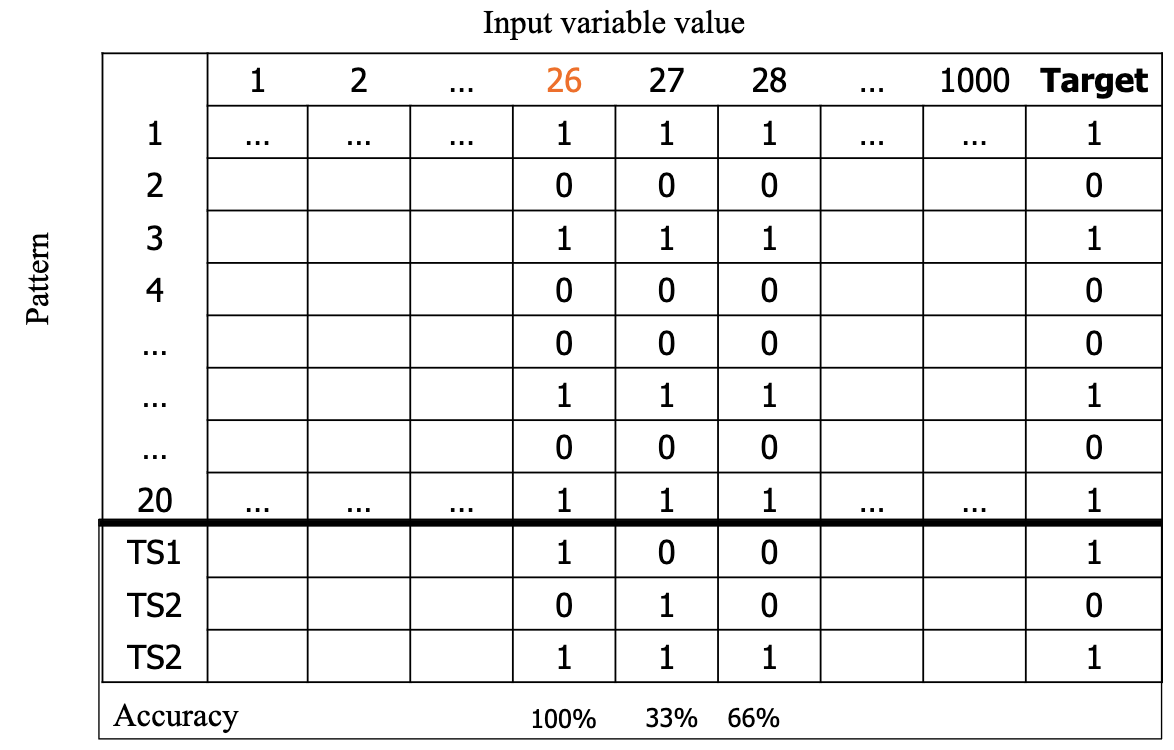
\includegraphics[width=0.5\linewidth]{img/table_counterex.png}
\end{figure}

\section{Grid Search}

Since hyperparameters are not learned by the learning algorithm, it's our task to find the best values for them. Choosing them is done by calculating the error on the validation set (VL). One way to search for hyperparameter values is to perform a grid search; candidates are generated from a grid of parameter values and tested on the validation set. This technique can have an high cost, since the total number of candidates is equal to $n^m$, where $n$ is the number of values in the range and $m$ is the number of hyperparameters. For this reason, grid search is typically used to fix some values in preliminary phases.

Additionally, we can perform two or more levels of nested grid search. First we apply a coarse search to a table with the combinations of all possible values set at intervals (e.g., growing exponentially) in order to find the best interval. Then we apply a second grid search by considering only the values withing that interval, and we can repeat the grid search until we perform a search fine enough for our needs.

There are alternatives to grid search, such as random search, automatized search, and many more offered by popular libraries.

\section{K-fold Cross Validation}

The most basic way of setting up data for model selection and model assessment is to split all of our data into three partitions (hold out cross validation). One of them will be the training set, one the validation set, and one the test set. However, it can be difficult to decide how to perform this split; it can depend on the complexity of the model, and signal-to-noise ratio. Also, how can we split the data so that each part is sufficiently sized? And can we avoid to perform a split that influences the results?

K-fold cross validation is another technique that can be used to split the data. Typically, the data is split into TR set and TS set. Then, k-fold cross validation is used over the TR set to obtain new partitions of the data to form different TR sets and VL sets. After finding the best hyperparameters, the model is retrained on the whole original TR set, and is assessed on the external TS set. Again, if the estimation is good enough, the model can be retrained on the test set data as well to produce the final model.

K-fold cross validation can still present some problems. It may be influenced by biases in the sample of data used. Cross validation can be repeated, by performing different splits with different random sampling; the estimation can be obtained by averaging the results. Another issue is having a sample too small to accurately represent the general population.

\section{Statistical Learning Theory}

\subsection{Vapnik-Cervonenkis Dimension}

The VC-dim (Vapnik-Cervonenkis dimension) is a measure of the complexity of a class of hypotheses $H$. It does not depend on the actual cardinality of the space, but on the number of distinct instances that can be completely discriminated (i.e., without error) using $H$.

Given $X$ an input space containing $N$ examples, and $H$ the hypothesis space, assume a binary classification task; there are $2^N$ possible \textbf{dichotomies} (i.e., partitions of the $N$ points either -1 or 1). A particular dichotomy is \textbf{represented} in $H$ if there exists an hypothesis $h$ in $H$ that realizes the dichotomy (it isolates all the points belonging to one class from the others).

\BoxDef{Shattering}{
The hypothesis space $H$ \textbf{shatters} $X$ if and only if $H$ can represent all the possible dichotomies on $X$.
}

\BoxDef{VC-dimension}{
The VC-dimension of a class of functions $H$ is the maximum cardinality of a configuration of points in $X$ that can be shattered by $H$.
}

If $VC(H) = p$, it means that there's at least an hypothesis in $H$ that shatters a configuration of size $p$, but cannot shatter any configuration of size $p+1$. If arbitrarily large (but finite) sets of $X$ can be shattered by $H$, then $VC$ is infinite. Note that there needs to be just one configuration of $p$ points that is shattered by an $h$; $h$ does not need to shatter all configurations of size $p$.

To make the concept clearer, consider an hypothesis space $H$ that is a set of lines ($h(x) = sign(wx + w_0) , \, x \in IR^2$). Each dichotomy is a different labeling of points as -1 or 1. This hypothesis space shatters some configurations of 3 points, such as the one shown in the figure below:

\begin{figure}[h]
    \centering
    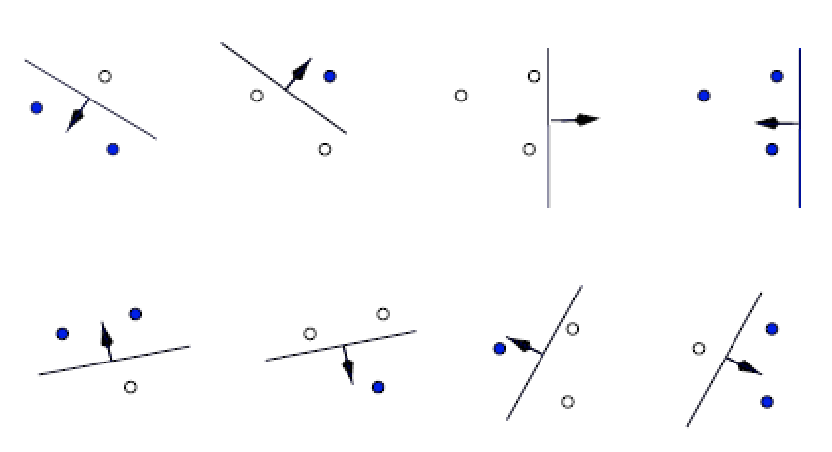
\includegraphics[width=0.5\linewidth]{img/shattering_1.png} 
\end{figure}
but cannot shatter this one:
\begin{figure}[h]
    \centering
    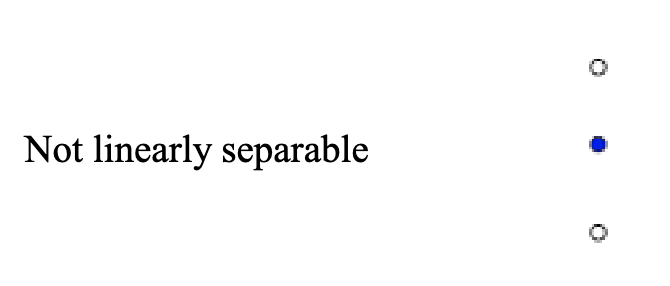
\includegraphics[width=0.5\linewidth]{img/Shattering_2.png}
\end{figure}\\
Still, its VC-dim is at least 3, since it can shatter at least the configuration on top. If we consider any configuration of 4 points, a single line cannot always separate them. This means that for any configuration of 4 points, there's at least a dichotomy that is not linearly separable, therefore the VC-dim is less than 4. In general, the VC-dim of a class of linear hyperplanes (LTU) in an $n$-dimensional space is $n+1$.

VC-dim is not the number of free parameters, although it is related. There exists models with only one free parameter and infinite VC-dim, such as K-NN. However, for many reasonable hypothesis classes the VC-dimension is linear in the number of free parameters of the model. Once we determine the VC-dim, we can then estimate the risk by defining an upper bound:

\begin{equation*}
    R[h] \leq R_{emp}[h] + \epsilon (VC,N,\delta)
\end{equation*}

The function $\epsilon()$ can be calculated in different ways depending on the task, class of functions, etc. This bound gives us a way to estimate the generalization error based only on training error and VC-dimensionality of $H$.

\subsection{Structural Risk Minimization}

SRM uses the VC-dimension as a control parameter to realize the best estimation of the generalization bound. Assume a nested structure of $n$ models/hypotheses space, such that: 

\begin{gather*}
    VC(H_1) \leq VC(H_2) \leq \dots \leq VC(H_n)
\end{gather*}

An example could be a nested structure of neural networks, where each $H_i$ corresponds to a network containing a different number of units; another could be polynomials with increasing degree.

The more the VC-dim increases, the more the VC-confidence and therefore the bound increase as well. The goal of SRM is to find the model corresponding to the trade-off on the bound between VC-dim and VC-conf. Once this bound has been determined, can it be used as an estimate of prediction errors? Yes, but rarely. It can be useful during model selection, but it's an overly pessimistic estimate for model assessment.